\documentclass{beamer}

%\usetheme{Madrid}
%\usetheme{Boadilla}
%\usetheme{default}
%\usetheme{Warsaw}
%\usetheme{Bergen}
%\usetheme{Frankfurt}
\usetheme{Darmstadt}

\setbeamercolor{normal text}{fg=white}
\setbeamertemplate{background canvas}[vertical shading] [top=black!95,bottom=black!65]

\definecolor{mypurple}{RGB}{207,78,64}
\usecolortheme[named=mypurple]{structure}

\definecolor{myorange}{RGB}{255,235,190}
\beamerboxesdeclarecolorscheme{orange}{orange}{myorange}

\definecolor{commandcolor}{RGB}{111,195,165}

\setbeamertemplate{footline}[page number]
%\setbeamercovered{transparent}
\setbeamercovered{invisible}
\setbeamertemplate{navigation symbols}{}

%\usepackage{musixtex}
\usepackage{multimedia}
\usepackage{graphicx}
\usepackage[utf8]{inputenc}
%\usepackage[T1]{fontenc}
\usepackage[french]{babel} 
%\usepackage[all]{xy}
%\usepackage{multirow}
%\usepackage{lmodern}
\usepackage{subfigure}
%\usepackage{ulem}
\usepackage{url}
\usepackage{hyperref}
\usepackage{verbatim}
\usepackage{xspace}
\usepackage{color}
\usepackage{xcolor}
\usepackage{rotating}
\usepackage{multicol}
\usepackage[export]{adjustbox}
\usepackage{textpos}
\usepackage{listings}
\usepackage{fontawesome}


\definecolor{mypurple}{RGB}{207,78,64}
\usecolortheme[named=mypurple]{structure}

\definecolor{myorange}{RGB}{255,235,190}
\beamerboxesdeclarecolorscheme{orange}{orange}{myorange}

\definecolor{dgreen}{RGB}{0,125,0}

\usepackage{tikz}
\usetikzlibrary{trees}

\setbeamertemplate{caption}[numbered] 

\newcommand{\setframetitle}[1]{\begin{center}
    \huge \textbf{#1}
\end{center}}


%% --------------

\title{Doxygen}
\subtitle{Atelier d'aide à la programmation}
\author{L\'eo \textsc{Baudouin}}
\institute{
  {\url{baudouin.leo @ gmail.com}}
}
\date{03-04 juin 2019}

%% --------------

\begin{document}

\begin{frame}
  \titlepage
\end{frame}

\section{Introduction}
\subsection{}

\begin{frame}{Doxygen}

\begin{center}

\includegraphics[width=0.3\linewidth]{images/doxygen-logo}
\end{center}

\begin{exampleblock}{Objectif}
\begin{itemize}
\item Documentation des fichiers C++
\end{itemize}
\end{exampleblock}

\begin{block}{Autres langages supportés}
\begin{itemize}
\item C, Objective-C, C\#, PHP, Java, Python, IDL, Fortran, VHDL, Tcl, D, \dots
\item Extension aux fichiers MatLab à l'aide d'un script en perl
\end{itemize}
\end{block}

\begin{block}{Format de sortie}
\begin{itemize}
\item HTML (compressé ou non), \LaTeX, RTF, PostScript, PDF
\end{itemize}
\end{block}
\end{frame}


\begin{frame}{Exemple de documentation}
\begin{block}{Objectif}
\begin{itemize}
\item \url{http://www.doxygen.nl/results.html}
\item \url{http://visp-doc.inria.fr/doxygen/visp-daily/classes.html}
\item \url{./libempty/build/doc/html/index.html}
\end{itemize}
\end{block}
\end{frame}

\begin{frame}{Fonctionnement}
\begin{center}
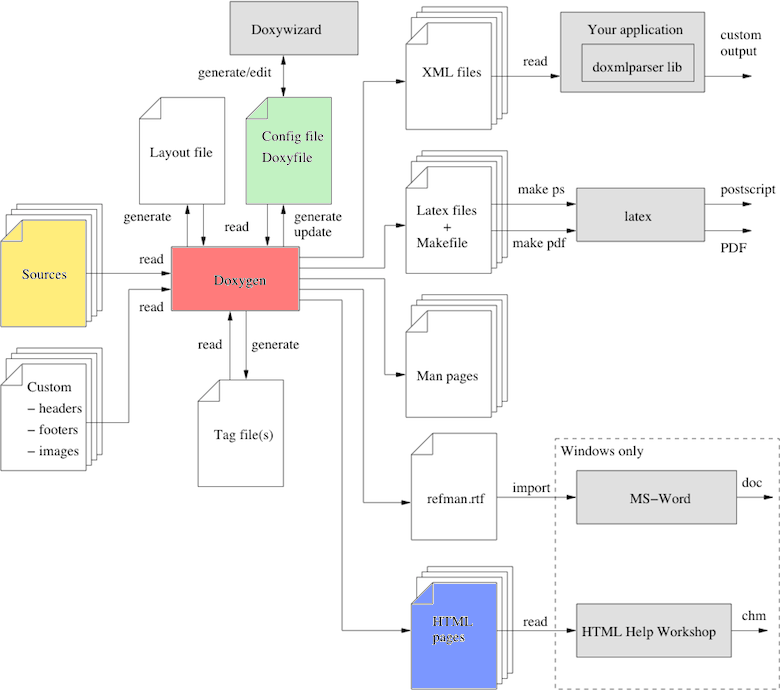
\includegraphics[height=0.9\textheight]{images/doxygen-flow2}
\end{center}
\end{frame}

\begin{frame}{Utilisation}
\begin{block}{Générer un Doxyfile}
\textcolor{commandcolor}{\verb?doxygen [-s] -g?}
\end{block}
\begin{block}{Compiler la documentation}
\textcolor{commandcolor}{\verb?doxygen Doxyfile?}
\end{block}
\begin{block}{Ouvrir la documentation}
\textcolor{commandcolor}{\verb?firefox doc/html/index.html \& ?}
\end{block}
\begin{block}{Interface graphique}
\textcolor{commandcolor}{\verb?doxywizard Doxyfile?}
\end{block}
\end{frame}

%-------------------------------------------------------------------


\section{Principes}
\subsection{}
\begin{frame}{Les commentaires}

\begin{columns}
\begin{column}{0.5\linewidth}
\begin{exampleblock}{Style C avec deux *}
/**\\
 * ... Documentation ...\\
 */\\
\end{exampleblock}

\begin{block}{Style Qt avec un !}
/*!\\
 * ... Documentation ...\\
 */
\end{block}
\end{column}
\begin{column}{0.5\linewidth}
\begin{block}{Style C++ avec trois /}
///\\
/// ... Documentation ...\\
///
\end{block}
\begin{block}{Style C++ avec un !}
//!\\
//! ... Documentation ...\\
//!
\end{block}
\end{column}
\end{columns}


\begin{block}{Autres styles}
\begin{scriptsize}
\url{http://www.doxygen.nl/manual/docblocks.html}
\end{scriptsize}
\end{block}

\end{frame}

\begin{frame}{Les tags}
\begin{block}{Ajouter un tag}
/**\\
 * \textcolor{dgreen}{\textbf{\textbackslash{}author}} Nom de l'auteur\\
 * \textcolor{dgreen}{\textbf{@author}} Nom de l'auteur\\
 */\\
\end{block}
\end{frame}


\begin{frame}{Ou placer les tags}
\begin{block}{N'importe ou}
Utiliser le tag correspondant au type de contenu :\\
/**\\
 * \textcolor{dgreen}{\textbf{@class}} ClassName\\
 * Description de la classe\\
 */\\
\end{block}

\begin{block}{Juste avant le contenu à documenter}
/**\\
 * Description de la classe\\
 */\\
 class ClassName\dots
\end{block}

\end{frame}

\begin{frame}{Ou placer les tags}
\begin{block}{Sur la ligne}
Utiliser le caractère : \textcolor{dgreen}{\verb?<?} :\\
int maVariable; /**\textcolor{dgreen}{\textbf{\verb?<?}} Description de la variable */\\
int maVariable; /*!\textcolor{dgreen}{\textbf{\verb?<?}} Description de la variable */\\
int maVariable; ///\textcolor{dgreen}{\textbf{\verb?<?}} Description de la variable \\
int maVariable; //!\textcolor{dgreen}{\textbf{\verb?<?}} Description de la variable \\
\end{block}

\begin{alertblock}{Attention}
Seulement pour les membres (d'une classe, d'un struct, \dots) et les paramètres (de fonction, macro, \dots)
\end{alertblock}

\end{frame}

%-------------------------------------------------------------------

\section{Tags fréquents}
\subsection{}

\begin{frame}{Les tags}
\begin{block}{Tags les plus utilisés}
\begin{itemize}
\item \textbf{\textbackslash struct} pour documenter une structure C.
\item \textbf{\textbackslash union} pour documenter une union C.
\item \textbf{\textbackslash enum} pour documenter un type énuméré.
\item \textbf{\textbackslash fn} pour documenter une fonction.
\item \textbf{\textbackslash var} pour documenter une variable/un typedef/un enum.
\item \textbf{\textbackslash def} pour documenter un \#define.
\item \textbf{\textbackslash typedef} pour documenter la définition d'un type.
\item \textbf{\textbackslash file} pour documenter un fichier.
\item \textbf{\textbackslash namespace} pour documenter un namespace.
\item \textbf{\textbackslash package} pour documenter un package Java.
\item \textbf{\textbackslash interface} pour documenter une interface IDL.
\end{itemize}
\end{block}
\end{frame}

\begin{frame}{Les tags}
\begin{block}{Tags les plus utilisés}
\begin{itemize}
\item \textbf{\textbackslash brief} pour donner une description courte.
\item \textbf{\textbackslash class} pour documenter une classe.
\item \textbf{\textbackslash param} pour documenter un paramètre de fonction/méthode.
\item \textbf{\textbackslash warning} pour attirer l'attention.
\item \textbf{\textbackslash author} pour donner le nom de l'auteur.
\item \textbf{\textbackslash return} pour documenter les valeurs de retour d'une méthode/fonction.
\item \textbf{\textbackslash see} pour renvoyer le lecteur vers quelque chose (une fonction, une classe, un fichier...).
\item \textbf{\textbackslash throws} pour documenter les exceptions possiblement levées.
\item \textbf{\textbackslash version} pour donner le numéro de version.
\end{itemize}
\end{block}
\end{frame}

\begin{frame}{Les tags}
\begin{block}{Tags les plus utilisés}
\begin{itemize}
\item \textbf{\textbackslash since} pour faire une note de version (ex : Disponible depuis la version 5.4.1).
\item \textbf{\textbackslash exception} pour documenter une exception.
\item \textbf{\textbackslash deprecated} pour spécifier qu'une fonction/méthode/variable... n'est plus utilisée.
\item \textbf{\textbackslash li} pour faire une puce.
\item \textbf{\textbackslash todo} pour indiquer un code "à faire".
\item \textbf{\textbackslash fixme} pour indiquer un code défectueux, "à réparer".
\end{itemize}
\end{block}
\begin{scriptsize}
Voir : \url{http://www.doxygen.nl/manual/commands.html}
\end{scriptsize}
\end{frame}

\begin{frame}{Formules}

\begin{itemize}

\item Formule dans le texte : entre deux \textcolor{red}{\verb?\textbackslash{f}\$?}

    \textcolor{cyan}{
    The distance between $(x_1,y_1)$ and $(x_2,y_2)$ is $\sqrt{(x_2-x_1)^2+(y_2-y_1)^2}$.}
    
\item Formule centrée non numérotée : entre \textcolor{red}{\verb?\textbackslash{}f[?} et \textcolor{red}{\verb?\textbackslash{}f]?}

    \textcolor{cyan}{
    $$ |I_2|=\left| \int_{0}^T \psi(t) \left\{ \int_{\gamma(t)}^a \frac{d\theta}{k(\theta,t)} \int_{a}^\theta c(\xi)u_t(\xi,t)\,d\xi \right\} dt \right| $$}
    
\item Utiliser un autre environnement que \textit{"math"} : entre \textcolor{red}{\verb?\textbackslash{}f\{environment\}?} et \textcolor{red}{\verb?\textbackslash{}f\}?} (ici \textbf{$environment = eqnarray*$})

    \textcolor{cyan}{
\begin{scriptsize}
    \begin{eqnarray*} g &=& \frac{Gm_2}{r^2} \\ &=& \frac{(6.673 \times 10^{-11}\,\mbox{m}^3\,\mbox{kg}^{-1}\, \mbox{s}^{-2})(5.9736 \times 10^{24}\,\mbox{kg})}{(6371.01\,\mbox{km})^2} \\ &=& 9.82066032\,\mbox{m/s}^2 \end{eqnarray*}
\end{scriptsize}
}

\end{itemize}
\end{frame}

\section{Exemple}
\subsection{}

\begin{frame}{Tag d'un fichier}
\begin{block}{Exemple}
\verb?/**?\linebreak
\verb? * @file calcul.c?\linebreak
\verb? * @brief Calculs simples?\linebreak
\verb? * @author L. Baudouin?\linebreak
\verb? * @version 0.0.1?\linebreak
\verb? * @date 26 avril 2014?\linebreak
\verb? *?\linebreak
\verb? * Effectue des calculs simples sur des variables.?\linebreak
\verb? *?\linebreak
\verb? * Addition: \textbackslash{}f\$ a = b + c\textbackslash{}f\$?\linebreak
\verb? *?\linebreak
\verb? */?
\end{block}
\end{frame}


\begin{frame}{Exemple}
\begin{exampleblock}{Voir le site}
\small
\url{http://www.doxygen.nl/manual/docblocks.html\#docexamples}
\end{exampleblock}

\begin{block}{En Python}
\small
\url{http://www.doxygen.nl/manual/docblocks.html\#pythonblocks}
\end{block}

\begin{alertblock}{Cloner le dép\^ot suivant}
\begin{small}
\url{https://github.com/lbaudouin/module-doxygen.git}
\end{small}
\end{alertblock}
\end{frame}


\begin{frame}{MatLab}

\begin{block}{Compiler la documentation}
\textcolor{commandcolor}{\verb?cd doxy-matlab?}\\
\textcolor{commandcolor}{\verb?doxygen Doxyfile?}
\end{block}

\begin{exampleblock}{Explications}
Le block de commentaire \textcolor{dgreen}{\textbf{\verb?///?}} est remplacé par \textcolor{dgreen}{\textbf{\verb?\%>?}} pour MatLab\\
Le fichier \textbf{m2cpp.pl} passe de la doc MatLab à une doc C++.\\
Le fichier \textbf{Doxyfile} configure la doc, il appelle \textbf{m2cpp.pl}
\end{exampleblock}

\end{frame}

\end{document} 

%-------------------------------------------------------------------

%\transdissolve[duration=0.25]
%
%\begin{exampleblock}{Avantages}
%\end{exampleblock}
%
%\begin{alertblock}{Inconvénients}
%\end{alertblock}
